\documentclass[8.01x]{subfiles}
\begin{document}

\chapter{Week 5: Homework 4}

\section{Problem 1: Oil drop}

``We release an oil drop of radius $r$ in air. The density of the oil is \SI{670}{kg/m^3}. $C_1$ and $C_2$ for 1 atmosphere air at $20^\circ$ C are $\SI{2.90e-4}{(kg/m)/s}$ and $\SI{0.82}{kg/m^3}$, respectively.

How small should the oil drop be so that the drag force is dominated by the linear term in the speed (in lectures we called this Regime I). In this regime, the terminal velocity is $(m g)/(C_1 r)$. [m is the mass of the drop].

$r \ll$ ...''

Well, there clearly isn't a truly ``correct'' answer here (estimates will vary), but we can use the definitions we have seen previously, which are that $v \gg v_{crit}$ means regime II, and $v \ll v_{crit}$ means regime I. The critical velocity $v_{crit}$ is when the force from each term is equivalent, which is at

\begin{align}
C_1 r v_{crit} &= C_2 r^2 v_{crit}^2\\
C_1 &= C_2 r v_{crit}\\
v_{crit} = \frac{C_1}{C_2 r} &\approx \frac{\num{3.54e-4}}{r} \text{ m/s}
\end{align}

The condition is then that the velocity is much, much smaller than this. Let's set up the terminal velocity in regime I (since the condition is that we must be way inside regime I, and the terminal velocity is the maximum one possible) one the left hand side of an equality, with the critical velocity on the other:

\begin{align}
\frac{m g}{C_1 r} &\ll \frac{C_1}{C_2 r}\\
\frac{4}{3} \pi \rho r^3 \frac{g}{C_1 r} &\ll \frac{C_1}{C_2 r}\\
r^3 &\ll \frac{3 C_1^2}{4 \pi \rho g C_2}\\
r &\ll \left(\frac{3 C_1^2}{4 \pi \rho g C_2}\right)^{1/3}\\
r &\ll \SI{1.54e-4}{m}
\end{align}

That's very small! $0.154$ mm, though the condition isn't just smaller than that, but \emph{much, much} smaller.

\section{Problem 2: Rough surfaces}

``An block of mass $m$, starting from rest, slides down an inclined plane of length $L$ and angle $\theta$ with respect to the horizontal. The coefficient of kinetic friction between the block and the inclined surface is $\mu_1$. At the bottom of the incline, the block slides along a horizontal and rough surface with a coefficient of kinetic friction $\mu_2$. The goal of this problem is to find out how far the block slides along the rough surface.

\begin{center}
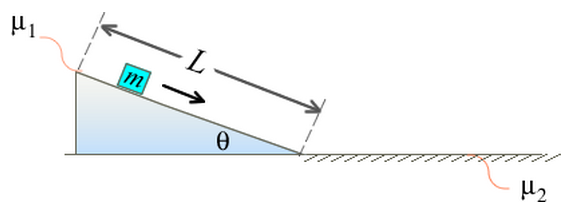
\includegraphics[scale=0.7]{Graphics/h4p2}
\end{center}

(a) What is the work done by the friction force on the block while it is sliding down the inclined plane?\\
(b) What is the work done by the gravitational force on the block while it is sliding down the inclined plane?\\
(c) What is the kinetic energy of the block just at the bottom of the inclined plane?\\
(d) After leaving the incline, the block slides along the rough surface until it comes to rest. How far has it traveled?\\
Express your answers in terms of $g$, $m$, $L$, $\theta$, $\mu_1$ and $\mu_2$.''

Now that we've learned about the conservation of mechanical energy, this problem should be easier to solve than it would be with basic kinematics and friction equations. The work done by gravity should be very easy to find: the work done by gravity is the change in potential energy, which is $m g h$ if we define $h$ to be the height at which the block starts out, and $y = 0$ to be at the ground, so that $U = 0$ there.

We thus need to find $h$. The illustration makes it look a bit as if the block starts a bit down the ramp, but I assume it travels the distance $L$, or this would be hard to solve indeed! Via trigonometry, $\sin \theta = h/L$ so $h = L \sin \theta$. That gives us, for the work done by gravity,

\begin{equation}
W_g = m g L \sin \theta
\end{equation}

... which answers part (b).\\
Next, we must find the work done by frictional forces as the block slides down. The magnitude of that force is

\begin{equation}
|F_f| = \mu_1 N = \mu_1 m g \cos \theta
\end{equation}

We decompose the normal force, since gravity is straight downwards, while the block is on an incline.\\
Since the force is constant, and work is force times distance, we can find the work easily as $W_f = |F_f| L$. However, let's keep track of the signs here! The frictional force is always opposing the motion relative to the surfaces, so it is ``backwards'' (to the left) while the block only moves to the right. Therefore, the work is negative:

\begin{equation}
W_f = -(|F_f| L) = - \mu_1 m g L \cos \theta
\end{equation}

... which answers part (a).\\
Next up is then the kinetic energy of the block as it has just reached the bottom (or end) of the incline. The kinetic energy started out at zero, and must now be at a maximum (since the potential energy is $U = 0$ at the bottom, by our definition). Without friction, it would be equal to the work gravity has done, but we must now add the work done by friction (subtract, in a way, since it is negative, but I prefer ``add'' to avoid confusion; subtracting a negative would give a larger value, which is clearly incorrect!).

\begin{align}
K = W_f + W_g &= m g L \sin \theta - \mu_1 m g L \cos \theta\\
              &= m g L (\sin \theta - \mu_1 \cos \theta)
\end{align}

The work-energy theorem at work... no pun intended.

Finally, part (d): how long does the block slide on the rough surface? It has a certain amount of kinetic energy, above; friction uses up a constant amount per unit length traveled, since it is constant at $\mu_2 N = \mu_2 m g$ (since the surfaces are now horizontal).

Using $d$ for the distance traveled, the work done by friction is then $\mu_2 m g d$ ($W = F d$). That work equals the initial kinetic energy, so we set them equal and solve for $d$:

\begin{align}
\mu_2 m g d &= m g L (\sin \theta - \mu_1 \cos \theta)\\
d           &= \frac{L (\sin \theta - \mu_1 \cos \theta)}{\mu_2}
\end{align}

That's all!

\section{Problem 3: Oscillating block}

``Consider an ideal spring that has an unstretched length $\ell_0 = \SI{3.1}{m}$. Assume the spring has a constant $k = \SI{36}{N/m}$. Suppose the spring is attached to a mass $m = \SI{7}{kg}$ that lies on a horizontal frictionless surface. The spring-mass system is compressed a distance of $x_0 = \SI{1.8}{m}$ from equilibrium and then released with an initial speed $v_0 = \SI{3}{m/s}$ toward the equilibrium position.

\begin{center}
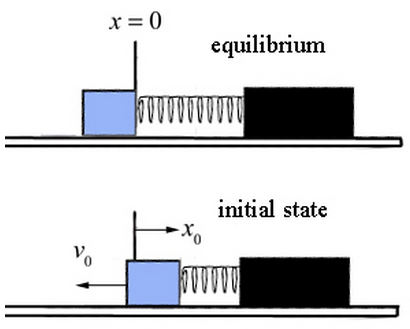
\includegraphics[scale=0.7]{Graphics/h4p3}
\end{center}

(a) What is the period of oscillation $T$ for this system?\\
(b) What is the position of the block as a function of time. Express your answer in terms of $t$.\\
(c) How long will it take for the mass to first return to the equilibrium position?\\
(d) How long will it take for the spring to first become completely extended?''

Since the spring is ideal, Hooke's law holds, and we can use the equations we found in lecture, by solving a differential equation for this simple harmonic oscillator. The equation we found was

\begin{equation}
x(t) = A \cos(\omega t + \varphi)
\end{equation}

where $A$ is the amplitude in meters, $\omega$ the angular frequency in radians/second, and $\varphi$ the phase angle in radians. $A$ and $\varphi$ are found from the initial conditions, while $\omega$ can be found as

\begin{equation}
\omega = \sqrt{\frac{k}{m}}
\end{equation}

The period of oscillation is

\begin{equation}
T = \frac{2 \pi}{\omega} = 2 \pi\sqrt{\frac{m}{k}} = 2 \pi \sqrt{\frac{7}{36}} \approx \SI{2.77}{s}
\end{equation}

To find the position as a function of time, we need to find the amplitude and the phase, by using the initial conditions. At $t = 0$, $x(0) = x_0 = 1.8$ meters, as given in the problem. We substitute those values into the $x(t)$ equation:

\begin{equation}
x_0 = A \cos(\varphi)
\end{equation}

That only gets us so far, since there are two unknowns, $A$ and $\varphi$. We can find a second equation in taking the time derivative of $x(t)$ to find $v(t)$, though, since we know the initial velocity.

\begin{align}
v(t) = \frac{dx(t)}{dt} = -A \omega \sin(\omega t + \varphi)
\end{align}

At $t = 0$, this should be equal to $-3$ (if $x_0$ is positive, then $+\hat{x}$ is towards the right, but $v_0$ is towards the left). Combined with the equation for $x(t)$, we have these two equations:

\begin{align}
x_0  &= A \cos(\varphi)\\
-v_0 &= -A \omega \sin(\varphi)
\end{align}

\begin{align}
-\frac{x_0}{v_0}  &= -\frac{\cos(\varphi)}{\omega \sin(\varphi)}\\
\omega \frac{x_0}{v_0}  &= \frac{1}{\tan \varphi}\\
\arctan \frac{v_0}{\omega x_0}  &= \varphi \approx 0.6338 \text{ rad} \approx \ang{36.31}
\end{align}

Solving for $A$ should now be dead simple, using the equation $x_0 = A \cos(\varphi)$:

\begin{align}
1.8 = 0.80578 A\\
A = \SI{2.23}{m}
\end{align}

$\omega$, using the formula above, is about $2.2678$ rad/s, so all in all, the formula for $x(t)$ is

\begin{equation}
x(t) = 2.23 \cos(2.2678 t + 0.6338)
\end{equation}

Evaluated at $t = 0$, this equals 1.7969 m, and the problem states $x_0 = \SI{1.8}{m}$ -- close enough; it's clearly due to rounding errors.

``(c) How long will it take for the mass to first return to the equilibrium position?''

That happens when $x(t) = 0$, so we set it up and solve for $t$:

\begin{align}
2.33 \cos(2.2678 t + 0.6338) &= 0\\
2.2678 t + 0.6338 &= \frac{\pi}{2} \text{ (by taking the arccosine of both sides)}\\
t &= \frac{\pi/2 - 0.6338}{2.2678} \approx \SI{0.413}{s}
\end{align}

``(d) How long will it take for the spring to first become completely extended?''

I assume that by ``completely extended'', they mean when it is as long as it will ever become -- since it is at its natural length at $x = 0$, which is what we found above. Since the initial velocity is in the ``extending direction'', this should happen the first time $v = 0$, so let's set the derivative, which we found earlier, equal to zero:

\begin{align}
-A \omega \sin(\omega t + \varphi) &= 0\\
-2.33 \cdot 2.2678 \sin(2.2678 t + 0.6338) &= 0\\
\sin(2.2678 t + 0.6338) &= 0\\
2.2678 t + 0.6338 &= \pi \text{ (by taking the arcsine of both sides)}\\
t &= \frac{\pi - 0.6338}{2.2678} \approx \SI{1.106}{s}
\end{align}

I chose $\pi$ instead of 0 for the arcsine because choosing 0 yields a negative time, which is clearly incorrect.\\
Honestly, I'm not completely happy with this solution, but it worked, at least.

\section{Problem 4: Spring block with friction}

``A block of mass $m = \SI{4}{kg}$ slides along a horizontal table when it encounters the free end of a horizontal spring of spring constant $k = \SI{16}{N/m}$. The spring is initially on its equilibrium state, defined when its free end is at $x = 0$ in the figure. Right before the collision, the block is moving with a speed $v_i = \SI{4}{m/s}$. There is friction between the block and the surface. The coefficient of friction is given by $\mu = 0.83$. How far did the spring compress when the block first momentarily comes to rest? Take $g = \SI{10}{m/s^2}$.''

\begin{center}
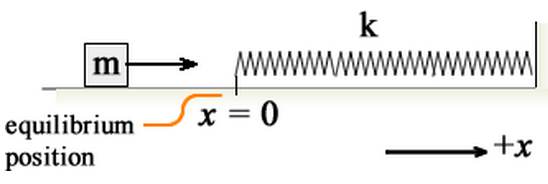
\includegraphics[scale=0.65]{Graphics/h4p4}
\end{center}

This problem can be conceptualized similarly to problem 2, i.e. conservation of energy. The block has an initial kinetic energy of $K = \frac{1}{2} m v_i^2$ = 32 joule; by definition, that kinetic energy must go down to $0$ when $v = 0$, which is of course when it first comes to a halt. Part of the kinetic energy will be eaten up by friction (turned into heat, mostly), and part will be transferred into the spring and stored there as potential energy.

The kinetic friction force is $\mu N = \mu m g$, which is constant regardless of position or velocity; the direction is opposite the motion, so to the left here, $-\hat{x}$. The spring's force is $-k x\ \hat{x}$, also to the left.

The work done by the forces together equals the sum of the forces times the distance $x$ the block travels; this work then equals the initial kinetic energy of the block. After having set the two equal, we can solve for $x$, which is how far the spring has compressed (and how far the block has traveled, after the ``collision'' with the spring). We can either set the sum of them equal to zero, or set the two work quantities equal, which is the same thing. I chose the latter:

\begin{align}
\frac{1}{2} m v_i^2 = x \left(\mu m g + k x\right)
\end{align}

Ah, but here's a snag: $k x$, the force from the spring, is not constant! It is 0 at the start, $k x$ only at the end of the motion, and somewhere in between for the rest of the time. \emph{However}, it is linear, which is good news for us! That means we can find the average force simply as $\frac{k x}{2}$, and keep going, with no calculus:

\begin{align}
\frac{1}{2} m v_i^2 &= x \left(\mu m g + 0.5 k x\right)\\
\frac{1}{2} m v_i^2 &= x \mu m g + 0.5 k x^2\\
\frac{m v_i^2}{k} &= 2 x \frac{\mu m g}{k} + x^2\\
x^2 + \frac{2\mu m g}{k} x - \frac{m v_i^2}{k} &= 0\\
\end{align}

Using the quadratic formula, $\displaystyle x = \frac{-b \pm \sqrt{b^2 - 4 a c}}{2a}$:

\begin{align}
x = -\frac{\mu m g}{k} \pm \frac{\sqrt{\left(\frac{2 \mu m g}{k}\right)^2 + \frac{4 m v_i^2}{k}}}{2}
\end{align}

If we stick some values into that mess, we find

\begin{align}
x = -2.075 \pm 2.88195
\end{align}

Since the answer is clearly positive as defined in the problem, it must be $x = -2.075 + 2.88195 = 0.80695 \approx \SI{0.807}{m}$.

\section{Problem 5: Half loop}

``A small bead of mass $m$ is constrained to move along a frictionless track as shown. The track consists of a semicircular portion of radius $R$ followed by a straight part. At the end of the straight portion there is a horizontal spring of spring constant $k$ attached to a fixed support. At the top of the circular portion of the track, the bead is pushed with an unknown speed $v_0$. The bead comes momentarily to rest after compressing the spring a distance $d$. The magnitude of the acceleration due to the gravitational force is $g$.

\begin{center}
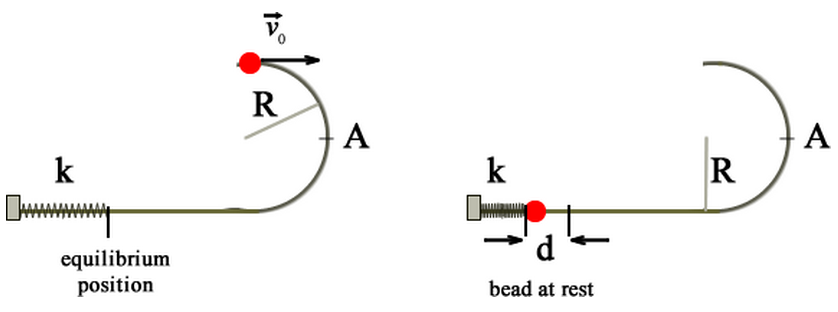
\includegraphics[scale=0.6]{Graphics/h4p5}
\end{center}

What is the magnitude of the normal force exerted by the track on the bead at the point A, a height $R$ above the base of the track? Express your answer in terms of $m$, $k$, $R$, $d$, and $g$ but \emph{not} in terms of $v_0$.''

Okay, let's see. There is no friction, so we should be able to rely on conservation of energy to find the initial velocity from the spring's compression. It is compressed a distance $d$, with a spring constant $k$. Now, unfortunately, I don't know how to calculate the stored potential energy in a spring; it's a common formula, easy to find -- but I would prefer to figure it out myself! Looking up a formula doesn't teach you much, but deriving it yourself can be very helpful indeed, especially if you've never seen it before.

So, let's take a sidestep for a moment.

\subsection{Potential energy stored in a spring}

Spring forces are conservative, so the amount of work done in compressing a spring should equal the amount of potential energy stored in it. We need to exert a force $F(t) = k x(t)$ to compress a spring, where $x(t)$ is the amount we have compressed it so far. The total work done, and the total energy stored, must therefore be the integral of this: 

\begin{align}
U_{spring} = \int_0^d F(t) \mathop{dx} = \int_0^d k x \mathop{dx} = k \Big[ \frac{x^2}{2} \Big]_0^d = k \frac{d^2}{2} = \frac{1}{2} k d^2
\end{align}

Neat! It looks a lot like the equation for kinetic energy (and many other equations in physics, for that matter).

\subsection{Back to the problem}

Now that we know how much energy is stored in the spring when the bead comes to a temporary halt, before being ``shot out'' again, we can find $v_0$, in case we need it later. The energy stored in the spring must come exclusively from the bead's kinetic energy (some of which come from gravity). If we define gravitational potential energy as 0 at the bottom, then it must be be $2 m g R$ at the top of the loop.

The spring starts out with no stored energy, while the bead starts out with its kinetic energy $\displaystyle K_E = \frac{1}{2} m v_0^2$ and its gravitational potential energy $2 m g R$. Since there is no friction or other resistive forces, the sum of all these must be conserved.

The speed at point A can be found by finding the bead's kinetic energy at that point, which is the sum of its initial kinetic energy and potential energy, minus the energy used up working against gravity, $m g R$, to reach point A:

\begin{align}
\frac{1}{2} m v_A^2 &= \frac{1}{2} m v_0^2 + 2 m g R - m g R\\
m v_A^2 &= m v_0^2 + 2 m g R\\
v_A &= \sqrt{v_0^2 + 2 g R}
\end{align}

We can find $v_0$. When the bead has compressed the spring fully, all of the initial kinetic energy plus all of the gravitational potential energy is now stored in the spring, so we can equate them:

\begin{align}
\frac{1}{2} m v_0^2 + 2 m g R &= \frac{1}{2} k d^2\\
m v_0^2 + 4 m g R &= k d^2\\
v_0^2 &= \frac{k d^2 - 4 m g R}{m}\\
v_0   &= \sqrt{\frac{k d^2 - 4 m g R}{m}}
\end{align}

$v_0^2$ is what we need to find $v_A$, however:

\begin{equation}
v_A = \sqrt{\frac{k d^2 - 4 m g R}{m} + 2 g R}
\end{equation}

Almost there! Now that we know the speed at A, we can apply the formula for centripetal acceleration, $\displaystyle |a_c| = \frac{v^2}{r}$, and then multiply by the mass $m$ to find the centripetal force.

The normal force from the track is the only possible source for this centripetal force, which is necessary for the bead to move along the (semi)circular track. Therefore, we find the centripetal force:

\begin{align}
N = m \frac{v_A^2}{R} = \frac{m}{R} \left(\frac{k d^2 - 4 m g R}{m} + 2 g R\right)
\end{align}

and that solves the problem!

\section{Problem 6: Full loop}

``An object of mass $m$ is released from rest at a height $h$ above the surface of a table. The object slides along the inside of the loop-the-loop track consisting of a ramp and a circular loop of radius $R$ shown in the figure. Assume that the track is frictionless.

\begin{center}
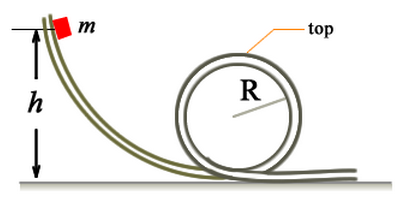
\includegraphics[scale=0.6]{Graphics/h4p6}
\end{center}

When the object is at the top of the loop it barely loses contact with the track. What height $h$ was the object released from? Express your answer in terms of some or all of the given variables $m$, $g$, and $R$.''

Well... Unless I'm missing something, I remember the answer from lecture! I'll still try to re-derive it, though, to make sure I fully understand the problem. If I do, this shouldn't take long.

Okay, so the track is frictionless, and we can use conservation of energy to simplify things. Since the object is released from rest, its initial potential energy is $m g h$, assuming $U = 0$ at $y = 0$; since that is my choice to make, I decide it shall be so.

When entering the loop, the potential energy is zero, and the object's speed is at a maximum, as is the kinetic energy. It then travels up $2 R$ against gravity, which causes it to lose kinetic energy again.

Let's first find the condition for the object not falling down at the middle of the loop. $|a_c| > g$ must be the case, or the object will not move in a circle. This puts a constraint on $v_{top}$, the speed at the top:

\begin{equation}
a_{c,top} = \frac{v_{top}^2}{R} \ge g
\end{equation}

Next, we need to figure out what $v_{top}$ is, as a function of the initial height $h$. At that height, it will have a potential energy of $m g 2 R$, which is smaller than the $m g h$ it begins with (or it will never reach that point).

\begin{align}
\frac{1}{2} m v_{top}^2 &= m g h - 2 m g R\\
v_{top}^2 &= 2 g h - 4 g R\\
v_{top} &= \sqrt{2g(h - 2 R)}
\end{align}

Now we just need to put the two together, and solve for $h$.

\begin{align}
\frac{2 g h - 4 g R}{R} &\ge g\\
2 g h &\ge 5 R g\\
h &\ge \frac{5}{2} R
\end{align}

Since the question is when it ``just barely'' loses contact, the answer is $\displaystyle h = \frac{5}{2} R$.

\section{Problem 7: Vertical spring}

``A spring of negligible mass, spring constant $k = \SI{99}{N/m}$, and natural length $\ell = \SI{1.3}{m}$ is hanging vertically. This is shown in the left figure below where the spring is neither stretched nor compressed. In the central figure, a block of mass $M = \SI{2}{kg}$ is attached to the free end. When equilibrium is reached (the block is at rest), the length of the spring has increased by $d_1$ with respect to $\ell$. We now lower the block by an additional $d_2 = \SI{0.4}{m}$ as shown in the right figure below. At $t = 0$ we release it (zero speed) and the block starts to oscillate. Take $g = \SI{9.81}{m/s^2}$.

\begin{center}
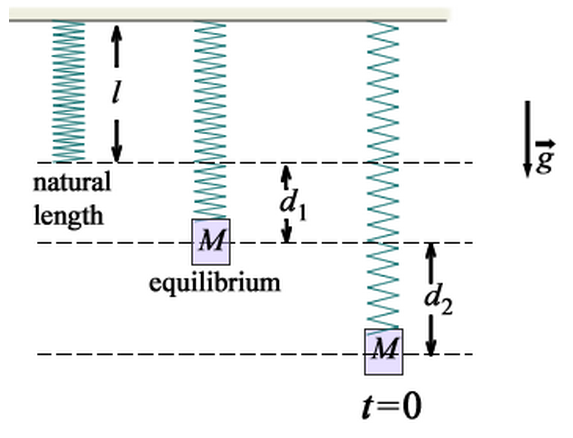
\includegraphics[scale=0.6]{Graphics/h4p7}
\end{center}

(a) Find $d_1$.\\
(b) What is the frequency (Hz) of the oscillations?\\
(c) What is the length of the spring when the block reaches its highest point during the oscillations?\\
(d) What is maximum speed of the block?''

I'll start off by finding $d_1$, not only because it's the first question, but because it should be independent of everything else.\\
For this problem, I choose a coordinate system of one axis, $y$, which is positive downwards, and has its origin at the spring's natural length. In other words, $y = + d_1$ when the system is at equilibrium with the mass.

Since it is in equilibrium, with the spring force upwards, and gravity downwards, with no acceleration:

\begin{align}
d_1 k &= m g\\
d_1 &= \frac{m g}{k} \approx 0.19818 \text{ m}
\end{align}

Now then, onto the rest of the problem. I will use the same coordinate system, by the way.

In a horizontal oscillator (as in lecture), there is only one horizontal force, which is that of the spring. I know (from a quick and dirty test) that the period is the same for this vertical oscillator, but how can we show that to be the case, now that gravity is present along the oscillating axis? If this were an exam question, I would \emph{not} have wasted a try on that assumption!

We can actually show that this system is equivalent to the horizontal one.\\
We've just shown that the ``new'' equilibrium position is at $y = d_1$. However, we can re-define $y$ instead, so that $y = 0$ at that point. Why? Because the block will oscillate around that point, moving equal amounts up as down from the new zero point, which is not the case for the old one. In other words, we will get a symmetrical problem if we change the zero point, so we do just that.

The spring force is upwards, in magnitude $k (d_1 + y)$ in this case, now. At $y = 0$, it should be $k d_1$, and for greater values of $y$ (further down), it should be greater, so that looks about right. Gravity is $m g$, always downwards. Putting this all together, $a = \ddot{y}$ being positive downwards, we set $m \ddot{y}$ equal to the net force, adding the downwards force (gravity) and subtracting the upwards force (spring force):

\begin{equation}
m \ddot{y} = m g - k(d_1 + y)
\end{equation}

However, note that since $d_1 = \frac{m g}{k}$, $m g = k d_1$, we can replace $m g$ by $k d_1$:

\begin{align}
m \ddot{y} &= k d_1 - k(d_1 + y)\\
m \ddot{y} &= - k y\\
\ddot{y} &= - \frac{k}{m} y
\end{align}
\begin{equation}
\ddot{y} + \frac{k}{m} y = 0
\end{equation}

A-ha! This is clearly the exact same differential equation we had earlier in lecture, only we call the axis $y$ instead of $x$, so we can safely use the same solutions! That it,

\begin{align}
\omega &= \sqrt{\frac{k}{m}}\\
T &= 2 \pi \sqrt{\frac{m}{k}}\\
y &= A \cos (\omega t + \varphi)\\
\dot{y} &= -A \omega \sin(\omega t + \varphi)\\
f &= \frac{\omega}{2\pi}
\end{align}

We have already solved (a), so let's calculate the frequency for part (b). Using the above formulas, we find $\omega \approx 7.03562$ rad/s, so $f \approx \SI{1.12}{Hz}$.

Next, the spring's length when the block reaches its highest point. The amplitude of the oscillation is $d_2$, the amount we extended it from the (new, with the mass) equilibrium point, so the answer is the spring's original length plus $d_1$, which is the new equilibrium point, minus the amplitude $d_2$. All in all, $\ell_{top} = \ell + d_1 - d_2 \approx \SI{1.098}{m}$.

Finally, the maximum speed of the block. The velocity is given by $\dot{y}(t)$ above, which is clearly maximized when the sine function is 1. We don't care when that happens, only that the speed at that point is the magnitude of the function's value when the sine term is 1, i.e. $A \omega = d_2 \omega \approx \SI{2.814}{m/s}$, and that's it for this question!

\section{Problem 8: Drag force at low speeds}

\begin{center}
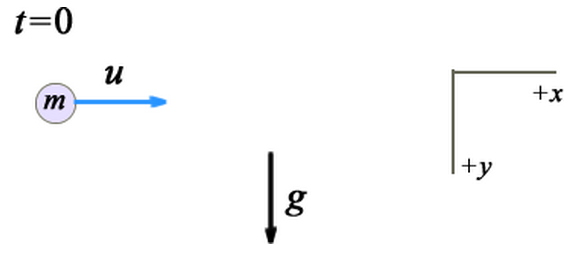
\includegraphics[scale=0.6]{Graphics/h4p8}
\end{center}

``At low speeds (especially in liquids rather than gases), the drag force is proportional to the speed rather than its square, i.e., $\vec{F} = -C_1 r \vec{v}$, where $C_1$ is a constant. At time $t = 0$, a small ball of mass $m$ is projected into a liquid so that it initially has a horizontal velocity of $u$ in the +x direction as shown. The initial speed in the vertical direction (y) is zero. The gravitational acceleration is $g$. Consider the Cartesian coordinate system shown in the figure (+x to the right and +y downwards).

Express the answer of the following questions in terms of some or all of the variables $C_1$, $r$, $m$, $g$, $v_x$, $v_y$, $u$ and $t$:

(a) What is component of the acceleration in the x direction as a function of the component of the velocity in the x direction $v_x$? express your answer in terms of $v_x$, $C_1$, $r$, $g$, $m$ and $u$ as needed.\\
(b) What is the acceleration in the y direction as a function of the component of the velocity in the y direction $v_y$? express your answer in terms of $v_y$, $C_1$, $r$, $g$, $m$ and $u$ as needed.\\
(c) Using your result from part (a), find an expression for the horizontal component of the ball's velocity as a function of time $t$? Express your answer in terms of $C_1$, $r$, $g$, $m$, $u$ and $t$ as needed (enter e\textasciicircum(-z) for $\exp(-z)$).\\
(d) Using your result from part (b), find an expression for the vertical component of the ball's velocity as a function of time $t$? Express your answer in terms of $C_1$, $r$, $g$, $m$, $u$ and $t$ as needed: (Enter e\textasciicircum(-z) for $\exp(-z)$).\\
(e) How long does it take for the vertical speed to reach 99\% of its maximum value? express your answer in terms of $C_1$, $r$, $g$, $m$ and $u$ as needed.\\
(f) What value does the horizontal component of the ball's velocity approach as $t$ becomes infinitely large? express your answer in terms of $C_1$, $r$, $g$, $m$ and $u$ as needed.\\
(g) What value does the vertical component of the ball's velocity approach as $t$ becomes infinitely large? express your answer in terms of $C_1$, $r$, $g$, $m$ and $u$ as needed.''

Wow! Okay, let's get started, I suppose. I will most likely use Mathematica for parts of this.

Anyway. The initial velocity in the $x$ direction is $u$, a given, while that in the $y$ direction is 0. In the $x$ direction, there is only the resistive force, acting towards the left, opposing the motion.\\
In the $y$ direction, there is gravity pulling the mass downwards, and a resistive force \emph{upwards}, slowing the ``fall''.

Newton's second law in the $x$ direction:

\begin{equation}
m a_x = m \ddot{x} = - F_{res_x} = - C_1 r v_x
\end{equation}

Any in the $y$ direction, with downwards defined as positive in the problem:

\begin{equation}
m a_y = m \ddot{y} = m g - F_{res_y} = m g - C_1 r v_y
\end{equation}

Well, at least they ask for stuff in one direction at a time, so we don't need to worry too much about having \emph{two} differential equations. Still, rearranged, they are

\begin{align}
&\ddot{x} + \frac{C_1 r}{m} v_x = 0\\
&\ddot{y} + \frac{C_1 r}{m} v_y - g = 0
\end{align}

Oh! This actually answers parts (a) and (b), I almost didn't notice. Just move everything except the $\ddot{x}$ or $\ddot{y}$ terms to the right-hand side, and those are the answers.

Next, they ask us for the velocity, as a function of \emph{time}. I think this means solving the differential equation, and then taking the derivative once (since the solution gives us the position).

Note that the differential equations involve $\ddot{x}$ and $\dot{x}$, or $\ddot{y}$ and $\dot{y}$, respectively, only we call the latter two $v_x$ and $v_y$, respectively. Therefore, these equations are \emph{not} identical to ones we've seen previously -- and they shouldn't be, as there clearly will be no oscillating motion in this case!

As far as I can tell, we have two second-order linear differential equations with constant coefficients. Honestly, I stuck this into Mathematica with $x(0) = x_0$ and $\dot{x}(0) = u$ as boundary conditions, differentiated the answer, and got

\begin{equation}
\dot{x} = u \exp\left(-\frac{C_1 r t}{m}\right)
\end{equation}

... which is marked as correct, and certainly looks plausible. I expected an exponential as a solution, and a decaying exponential that starts out at the initial velocity surely is a reasonable solution.

Next, onto the $y$ direction. Same deal, solve differential equation with boundary conditions ($y(0) = y_0$, $\dot{y}(0) = 0$), differentiate, simplify:

\begin{equation}
\dot{y} = \frac{m g}{C_1 r} \left(1 - \exp\left(-\frac{C_1 r t}{m}\right) \right)
\end{equation}

With the one minus the exponential there, we get an equation that grows up to $\displaystyle \frac{m g}{C_1 r}$ after a certain time, dictated by the term $\displaystyle \frac{C_1 r}{m}$.

For part (e), we can set the multiplying term, $1 - \exp(...)$ equal to $0.99$ and solve for $t$ to find the answer:

\begin{align}
1 - \exp\left(-\frac{C_1 r t}{m}\right) &= 0.99\\
-\frac{C_1 r t}{m} &= \ln(0.01)\\
\frac{C_1 r t}{m} &= \ln(100) 
\end{align}

The last step is because $\ln(0.01) = \ln(1/100) = \ln (1) - \ln(100) = -\ln(100)$, and the minus signs then cancel from both sides. Moving on...

\begin{equation}
t = \frac{m \ln(100)}{C_1 r}
\end{equation}

And finally, the limits of the velocities as $t$ becomes infinitely large. We don't need no calculus for this one, just common sense. The $x$ velocity has a force opposing the motion, proportional to the speed. It will reduce the motion until there is none, and then disappear; so $v_x = 0$ as $t \to \infty$.

As for $v_y$, the ``multiplying term'' above goes to $1$ as $t \to \infty$, so the velocity goes to $\displaystyle \frac{m g}{C_1 r}$.

That's it for this week!

\end{document}
